In this chapter, we acquaint ourselves with the question of forecasting dynamical systems with unknown underlying structures, state and discuss the shortcomings of the Takens delay embedding theorem and discuss various issues faced while forecasting. 

Consider a relatively simple learning problem: 
Given the sequence $(u_0, u_1, \ldots, u_m)$ for $m\in\mathbb{Z}$, a finite segment of an orbit of the map $T$ where $T$ is defined by the update equation $u_{n+1} = Tu_n$, forecast the values $u_{m+1}, u_{m+1}$ where the map $T$ is unknown, given that $u_m$. 

A practical example of this would be the subsequent scenario: given the time-sequential coordinates of an object moving in space, predict the future positions of that object. We are very rarely, if at all, presented with a problem where the entire state information is available to us in the form $u_n$ at some timestep $n\in\mathbb{N}$. Consider then a more complicated learning problem:

Suppose we only have the observations $\theta(u_0), \theta(u_1), \ldots, \theta(u_m)$ of the true system states $u$ in an unknown dynamical system $(U,T)$ and we wish to predict the values $\theta(u_{m+1}), \theta(u_{m+2})$ and so forth.

First we establish the method of Takens delay embedding. 
In this method, one considers a discrete-time dynamical system defined on a 'nice' space (a smooth manifold)\ednote{B: Should this be further explained?} that can be obtained as time-$K$ map of a continuous time-dynamical system, concepts formalised below.
We make observations from such a system, i.e., we observe the evolution of $\theta(w_0)$ (where $w_0$ represents the initial state) by examining  a finite set of values of $u_n :=  \theta(w_n) = \theta(Tw_{n-1})$. The sequence $\{u_n\}$ represents a scalar time-series and intuitively $\theta$ represents a probe inserted into a bigger system which is itself only measuring/extracting a small part of the greater system state at time $t=n$. 
Consider, for example, a thermometer erected to measure the ambient temperature in a local village. This measurement function, the thermometer, is capturing only a single aspect, the temperature, of a much grander dynamical system entailing the current weather of the surrounding area. Even more than that though- it is measuring a miniscule part of the global weather system. 


%Given the sequence $\{u_1, u_2, \ldots, u_n}$, we define the variable \newline $y_n:=[\theta_n, \theta_{n-\tau}, \ldots, \theta_{n-(2d-2)\tau}, \theta_{n-(2d-1)\tau}]^{T}\in\mathbb{R}_{d}\times{1}$ where $\tau$ represents the lag and $d$ the dimension of the attractor. (We shall return to these terms shortly and their discussion may be put on hold for the time being).

However, the actual state $u$ of a system is seldom, if ever, fully known. the most one can do is to insert probes into a system to obtain partial information through the measurements taken. Moreover, the process of taking a measurement itself introduces two additional aspects which complicate the problem: \ednote{B: Perhaps this edit makes more sense? M: Maybe replace difficulty by saying that we need to consider two aspects. }
\vspace{-8mm}
\begin{enumerate}[noitemsep, label=\roman*.]
  \item A series of measurements over a specific time interval is inherently a discretisation procedure of the underlying continuous-time dynamical system. (Hence why we restricted our attention to discrete-time systems in the preceding section)
  \item A probe will never be entirely accurate, and so the act of measurement introduces a certain measure of numerical noise/inaccuracy.
\end{enumerate}



From here we construct a multidimensional observable using the method of stacking previous observations, i.e., we create delay-coordinate map defined by
$\Phi_{k,\theta}(w) := (\theta(T^{-k}w)\ldots,\theta(T^{-1}w),\theta(w))$.  
The concept of an observable is understood in the sense of an observable as originally introduced by~\cite{takens1981detecting, genericObservableAeyels} to refer to a probe or measurement function inserted into the system. 
Takens' theorem, in essence, refers to the fact that for a sufficiently large $k$, we can define a dynamical system on the space $\mathbb{R}^{k+1}$ with states $\Phi_{k,\theta}(w)$, $\Phi_{k,\theta}(Tw)$, $\Phi_{k,\theta}(T^2w)$, etc. This dynamical system is topologically conjugate to the unknown underlying system $(W,T)$. We recall the Takens delay embedding theorem next.


%We may then ask ourselves the question: Is it in any way possible to retain information about the system state $x(t)$ in this temporal data-series $\theta(x(t))$? The answer is easily yes if T is known. However, neither this, nor even the exact function $\theta$ is available. 

\section{Takens Embedding Theorem}\label{sect_Takens}

We define first the concepts of homeomorphism and embedding:
\begin{Definition}\rm
  [\bf {Homeomorphism}]\label{Dfn_homeo}\rm
  A homeomorphism is a function $f:Z\rightarrow Y$ between two topological spaces $Z$ and $Y$ that is continuous, bijective and has a continuous inverse. 
\end{Definition}

\begin{Definition}
  [\bf {Embedding}]\label{Dfn_embed}\rm
  Consider a homeomorphism $f:Z\rightarrow Y$ for $Y\subset X$. $Z$ is said to be embedded in $X$ by $f$.
\end{Definition}

Takens Theorem states a result establishing a relationship between the observed and underlying dynamical systems by showing that the concatenation of a sufficiently large number of previous observations into a vector will, under certain conditions, generate a map between the vectors from the respective systems.  We formulate the theorem from \cite{takens1981detecting}.  

\begin{Theorem} 
	[\bf Takens Embedding Theorem (adopted from \cite{takens1981detecting}] \label{Thm_Takens}
         Let $W$ be a compact manifold of dimension $m$, and $d\ge m$ so that $2d$ is an integer. It is a 
            generic property for the pair $(T, \theta)$,  where $T:W \to W$ is
            a smooth diffeomorphism, and $\theta:W \to \mathbb{R}$ a smooth function, the map $\Phi_{2d,\theta}:W \to \mathbb{R}^{2d+1}$ defined on $W$ by 
            $\Phi_{2d,\theta}(w) := (\theta(T^{-2d}w)\ldots,\theta(T^{-1}w),\theta(w))$
            is a diffeomorphic embedding; by `smooth' we mean at least $C^2$. Consequently, there exists a map $F_\theta: \Phi_{2d,\theta}(W) \to \Phi_{2d,\theta}(W)$ defined by $$F_\theta: (\theta(T^{-2d}w),\ldots,\theta(T^{-1}w),\theta(w)) \mapsto 
            (\theta(T^{-2d+1}w),\ldots,\theta(w),\theta(Tw))$$
           so that $(W,T)$ is topologically conjugate to 
            $(\Phi_{2d,\theta}(W), F_\theta)$.    
\end{Theorem} 

By generic we mean a residual set on a certain topology on appropriate spaces of functions (that we do not describe here) \ednote{B: Where can I find a citation for this?}. 
By $C^2$, we make reference to a twice-differentiable function  with a continuous second derivative. In our scenario (and this remains important throughout) the input space $U$ is considered the attractor.~\label{attractor_U}

Below we reproduce Figure 1 from \cite{Supp}.

%Some explanation is beneficial. Takens establishes a delay-coordinate map $\Ftheta$ defined in \ref{eqn_takens} for $T$ the flow (\ref{defn_flow}) defined by the update equation  $Tu_n=u_{n+1}$ and $theta$ our measurement function. When confining a dynamical system to the manifold U (in which the underlying system is contained), Takens showed that if certain smoothness conditions are satisfied on $T$ and $\theta$, then the delay-coordinate map $\Ftheta$ embeds $U$ in the reconstruction space $R^{2d+1}$ \textbf{we haven't used the term reconstruction space yet, so this is falling out of the blue}, for almost every choice of measurement function $\theta$, the observable. By almost every choice here, we mean that we exclude some observations which do not give any information. To see a more precise discussion, see \textbf{xxx} for we do not concern ourselves with a further elaboration on this report.

%Alternatively we may also make the statement: Takens' Embedding Theorem guarantees that almost all dynamical systems can be reconstructed from just one noiseless observation sequence \textbf{this isn't obvious from the theorem's formulation, is it?} i.e. for a great number of possible observation functions $\theta$, $\Ftheta$ preserves the topology of U. \textbf{'preserving the topology' is not something we've touched on before. Perhaps I should add to previous discussion so logic flows seamlessly here}.

\begin{figure}[ht]
  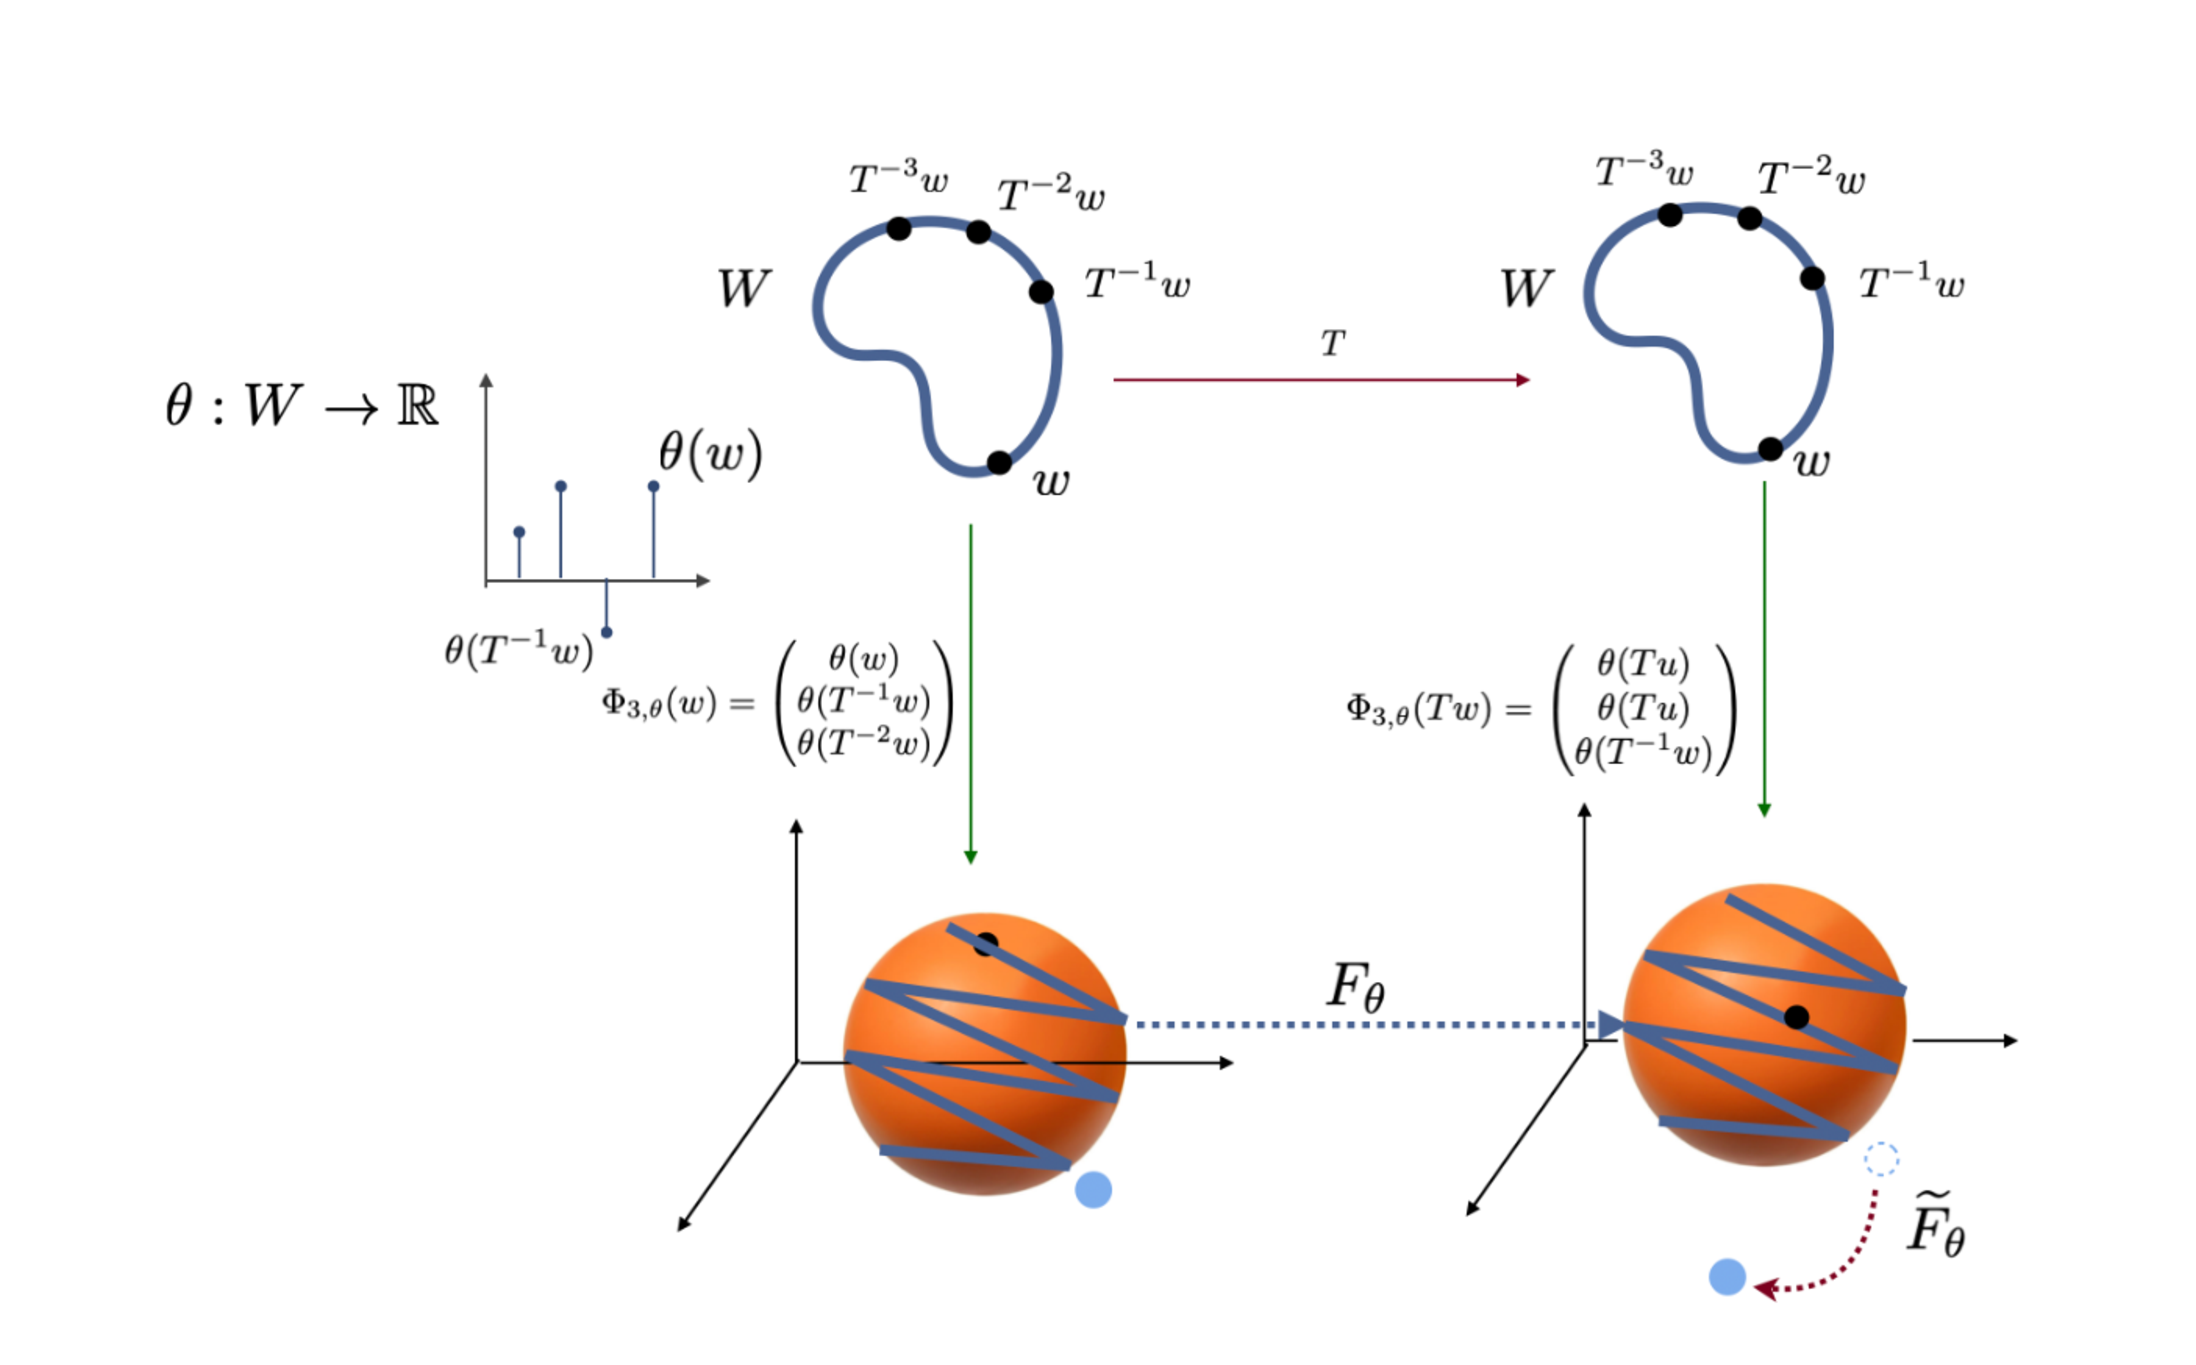
\includegraphics[scale=0.25]{Graphs/_takensmap.eps}
  \centering
  \captionof{figure}{Schematic of Takens Embedding Theorem's usage and impact of iterates slipping from the attractor when the approximation $\tilde{F}_\theta$ of $F_\theta$ is learnt.}
  \label{fig:takensmap}
\end{figure}

If we can learn the map $F_\theta$, from sufficient number of data points of $\{\phi_{2d,\theta}(w_n)\}$, then we also know how to forecast how $\theta(w_n)$. 


%Once again we pause and consider the graph to consolidate our understanding of the conjugacy (\textbf{are we being too simplistic?}). If we are in state $u$ and then evolve towards state $Tu$ before embedding into $\mathbb{R}^{2m-1}$, then this is equivalent to first embedding into $\mathbb{R}^{2m-1}$ and then evolving through the map $\Ftheta$, i.e. $\Phi_{2d,\theta}\circ{F}_{\theta} = T\circ\Phi_{2d,\theta}$. The map $F_theta$ is a homeomorphism as well. 

%Thus information about U can be retained in the time series' (or observation's) output. By preserving the topology on the manifold $U$ in the reconstruction space $X$ (\textbf{not discussed before}), we are also guaranteed the preservation of topological invariants of the manifold, of which dimensionality is one such invariant. (We note here that dimensionality will again be considered later in this project).

\section{Practical Limitations to Takens' Theorem}
Takens' Embedding Theorem is a powerful result, and it provides compelling reason to believe that one could conceivably reconstruct a system conjugate accurately to the underlying system. 
Nonetheless, it does present some severe practical limitations:
\vspace{-5mm}
\begin{enumerate}
\item Even supposing that we could indeed find $F_\theta$ , our \emph{approximation} of  $F_\theta$ is a map from a larger set $\mathbb{R}^{2d+1}$ containing the embedded attractor. There are, however, no theoretical guarantees that $F_\theta$ will retain  $V=\Phi_{2d,\theta}(W)$  as an attractor although $W$ could itself be an attractor.
\item Takens theorem is stated only for noiseless observations. Due to noise $\epsilon_n$ the delay vector $\Phi_{2d,\theta}(w_n) + \epsilon_n$  may lie outside $V$.Furthermore, due to the chaotic nature of the underlying system (i.e. the fact that it has SIDC), the evolution of $\Phi_{2d,\theta}(w_n) + \epsilon_n$ under the map $F_\theta$ could move out of $V$ completely. This problem can be overcome  by using a driven dynamical system with some properties, and we discuss this in Chapter\ref{ch3}. 
\end{enumerate}

% The Takens embedding theorem does not guarantee global dissipativity.
% \ednote{B:Links with~\ref{subs_LearnGamma} in discussion of dissipativity of $\Gamma$.  Sir, I'm not sure how to write this here - I think it a beneficial point to make so as to set the stage for the later discussion in ~\ref{subs_LearnGamma}, but I am unsure there as well.}


Though not a uniquely related to the Takens embedding theorem, we do opt to make mention of another requirement for our work. 
The methods described here are applicable for data originating from a surjective map. 
This follows from the fact that when $T$ maps the space $U$ into a proper subset $B$ of$ $U, there exists some point in $U - A$ that does not have a preimage and we conclude that $T$ is not surjective. 
An example of this would be the case when a system displays energy-loss. Consider, for instance, consider the dying oscillations for a damped pendulum. (An account of greater depth  is provided in~\ref{ch5})

This requirement is not overly restrictive, as a great number of chaotic systems do have a surjective map. (Cite) \ednote{B: I remember you saying this in one of our sessions, but don't have a source for it. Do you have a specific reference?}

